% \noindent

\subsection{Bewertungskriterien}

\todoin[color=NOTES]{
Kriterien: \break
- Perfomance (Schnelligkeit) --> Durch Layer 2 Lösungen (z.B. Lightning Network) (recht) hoch, ansonsten durch privates System (dann aber nicht dezentral und so Sicherheitsrisiken) \break
- Skalierbarkeit --> Durch Layer 2 Lösungen (z.B. Lightning Network) möglich \break
- Sicherheit (u.a. AuditLog) --> Wenn öffentliches System, dann generell durch Implementeirung beeinflusst, ansonsten durch privates System wie jetzt \break
- Transparenz --> In öffentlichem System sehr hoch, ansonsten durch privates Systeme wie jetzt \break
- Privatsphäre --> In öffnetlichem System quasi nicht möglich (evtl. durch HD-Wallets), ansonsten durch privates System (dann aber nicht dezentral und so Sicherheitsrisiken) \break
- Kosten  \break
- Komplexität (Aufwand, Wartung, ...) --> Erstmal Aufwand, dann aber gringer (vor allem wenn nur ein System verwendet wird, im Gegensatz zur aktuellen Situation) \break
- Erweiterbarkeit (z.B. neue Anforderungen) --> Durch Proxys möglich \break
}

\todoin[color=NOTES]{
    Ist-Zustand: \break
Quelle: Persönliches Gespräch mit Nils Pudenz (OE-4293) \break
Portal (Sparkassenmitarbeiter) \break
Online-Banking (Sparkassenkunde) \break
Cobol-Job \break
$\downarrow$ \break
OSPE-Services \break
$\downarrow$ \break
DOING 1 - N \break
$\downarrow$ \break
Inhausclearing: DiBus (Quelle: Gespräch Christian Krauthoff (OE-4293)) \break
Inland / SEPA: Clearing / TARGET / SWIFT \break
Ausland: Clearing / SWIFT \break
\break
"Eigentliche Idee von Cobol wegkommen --> Neues Projekt (AZV) nun aber 80\% Cobol" \break
\break
\break
\break
Fragen:\break
- Wie wird sichergestellt das nur der Inhaber eines Kontos Buchungen durchführen kann? \break
- Wie wird sichergestellt, dass die Datenbank mit den Kontodaten nicht manipuliert werden kann? \break
- Kosten für Transaktionen / Kontoführung generell? \break
Osplus produktkatalog \break

- Wie wird der Zugang zur Prod-DB geregelt? \break
\break
\break
\break
Sicherheitsaspekte: \break
- Code Review durch unabhängige Entwickler (also welche die nicht am Projekt mitgearbeitet haben), Quelle: Gespräch mit Paulina Rave (OE-4295) \break
- Automatische Codeprüfung, Quelle: Gespräch mit Paulina Rave (OE-4295) \break
- GPS (Geschäftsprozesse), die die Verwendung von Daten in einem bestimmten Kontext klar definieren, Quelle: Gespräch mit Paulina Rave (OE-4295) \break
}

\todoin[color=NOTES]{
Quelle: Wiki - Richtlinie Geschäftsprozesse \break
Unterhalb dieser Seite finden Sie eine Artikel zum Thema Geschäftsprozesse. Unter "Geschäftsprozess" sind hier die mit der Anwendung GPA erstellten Abläufe durch eine Verkettung von Aktivitätstypen zu verstehen. Diese Geschäftsprozesse werden durch die GPS ausgeführt, um ein bestimmtes geschäftliches oder betriebliches Ziel zu erreichen.
Die Beschreibungen der untergeordneten Seiten haben jeweils einen unterschiedlichen Charakter und dienen der Information oder stellen Richtlinien für die Entwicklung, den Test und die Ausführung von Geschäftsprozessen dar. Details finden Sie jeweils auf den einzelnen Seiten.
Die Seiten werden fortlaufend im Rahmen eines OSPlus-Releases und der Weiterentwicklung der Anwendungen GPA und GPS (siehe Glossar) aktualisiert.
Untergeordnete Seiten:
}

\subsection{Ist-Zustand}
\label{sec:ist-zustand}
Aktuell läuft die Abwicklung des Zahlungsverkehrs der Sparkassen über einen Großrechner (Mainframe) von IBM.\footappendix{Vgl. hierzu und zum Folgenden}{i1:f4}
Für den Großrechner werden sogenannte „Jobs” - also Kurzprogramme, die eine bestimmte Aufgabe erfüllen - geschrieben. Dafür wird die Programmiersprache COBOL verwendet, welche hoch performant ist und so die Massendatenverarbeitung ermöglicht.
Allerdings sind COBOL-Jobs an den Großrechner gebunden und immer weniger Entwickler sind in der Lage, diese zu schreiben.
Daher werden zusätzlich Java-Jobs geschrieben, die ebenfalls auf dem Großrechner laufen, aber auch auf anderen Systemen ausgeführt werden könnten.
Es ist das Ziel, vor allem die Verwendung von COBOL-Jobs - aber auch die Verwendung vom Großrechner im Allgemeinen - zu reduzieren und so auf andere Systeme zu migrieren.
Neuentwicklung haben die klare Richtlinie in Java implementiert zu werden und nur kritische Themen - im Sinne von Zeit und Datenmasse - auf dem Großrechner zu belassen.\footappendix{Vgl. Persönliches Gespräch mit Nils Pudenz - Entwickler AZV \& ZV-Rekla (OE-4293);}{i1:f4}
Es können teilweise 2 Millionen Transaktionen in ca. 20 Sekunden durchgeführt werden oder mehrere Jobs parallel laufen.
Für weniger kritische Themen werden OSPE-Services verwendet, die auf einem anderen System laufen.
Grundsätzlich laufen Prozesse des Zahlungsverkehrs wie folgt ab:

\begin{figure}[ht]
    \centering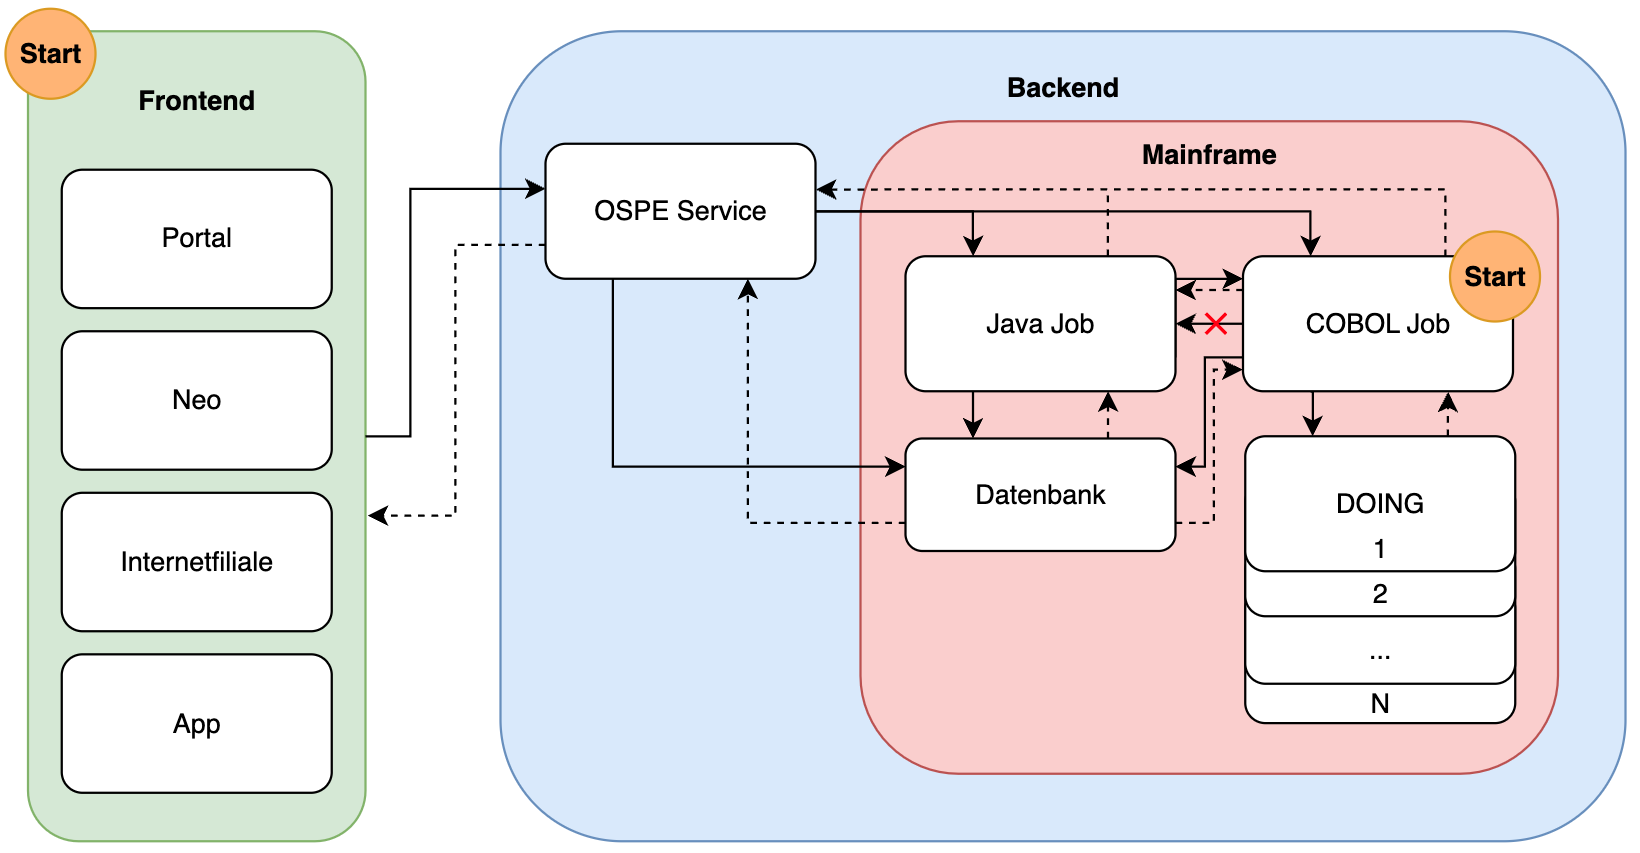
\includegraphics[width=0.9\textwidth]{Abbildungen/OSPlus-Diagramm.png}
    \caption{OSPlus-Diagramm}
\end{figure}

\todo[color=REVIEW]{Itemize notwendig? Ja, bitte}
\begin{itemize}
    \item Ein Mitarbeiter oder ein Endkunde setzt einen Prozess im Frontend in Gang (bspw. Überweisung oder Abfrage eines Kontostands).
    Dies kann über das Portal oder die Neo-Anwendung für Mitarbeiter oder das Online-Banking / die App für Endkunden geschehen.

    Ein Prozess kann ebenfalls durch einen COBOL-Job in Gang gesetzt werden (bpsw. bei Terminüberweisungen).
    \item Die Anfrage wird von einem OSPE-Service verarbeitet.
    Entweder kann dieser die Anfrage direkt (in in Verbindung mit anderen OSPE-Services) bearbeiten oder er ruft einen Java- oder COBOL-Job auf.
    \item Der Java-Job kann ebenfalls COBOL-Jobs aufrufen, andersherum ist dies nicht möglich.
    \item Bei bestimmten Prozessen (bpsw. Transaktionen) müssen eine Anzahl an Prüfungen - die DOINGs - durchgeführt werden. 
    (Z. B., ob die IBAN existiert, ob der Kontoinhaber der richtige ist, ob das Konto gedeckt ist oder auch, ob der Empfänger auf einer Sperrliste steht.) 
    \item Ist diese Prüfung erfolreich, kann der Prozess fortgesetzt werden.
    \item Sowohl die OSPE-Services als auch die Java- und COBOL-Jobs greifen auf die Datenbank zu, um die benötigten Daten zu erhalten bzw. zu speichern. 
\end{itemize}

Kostentechnisch ist es schwer, die Kosten pro Transaktion zu bestimmen, da es sich hierbei um Volumentverträge handelt.
Den Sparkassen werden 1,00 € bis 1,50 € pro tausend Zahlungsein- oder -ausgängen berechnet.\footnote{Vgl. interne Preisliste OSPlus 2024.}

\bigbreak
\bigbreak

\noindent
Um Daten nachvollziebar zu speichern - also so, dass auch nach Änderung oder eigentlicher Löschung noch der vorherige Stand ermittelbar ist -, werden Daten nie wirklich aktualisiert oder gelöscht, sondern es wird ein neuer Datensatz angelegt, der den aktuellen Stand der Daten enthält.
Der alte Stand wird nur „deaktiviert”, also mit einem Ablaufdatum versehen, sodass dieser nicht mehr verwendet wird.\footappendix{Vgl. hierzu und zum Folgenden}{i1:f2}
Erst nach einer in der DSGVO festgelegten Zeit - im Falle von Kontodaten sind dies 10 Jahre - kann dieser Datensatz dann wirklich gelöscht werden.



\todo[color=REVIEW]{Evtl. noch GPS erklären?}